


\documentclass[main]{subfiles}

\begin{document}

\chapter{Background Research}

\section{Scope of Research} \label{sec:scoperesearch}

In Chapter 1 (``Approaches to Interpretability'') a brief overview of feature attribution methods was provided with reference to a distinction between model-specific and model-agnostic methods. This is a common distinction in the literature and was also used to guide research in this project. The panel of methods chosen for evaluation ultimately consisted of a balanced selection from both approaches. 

A major difficulty of this project was distilling the broad literature on these methods however. For the model-specific (neural network) family, different angles are commonly taken to calculate feature ``relevance'' or importance. These include generally:
\begin{itemize}
\item \textbf{Backpropagation-based} methods or `importance signal' projections (such as activations in a hidden layer)
\item \textbf{Gradient-based} methods, saliency maps and output sensitivity methods
\item \textbf{Perturbation-based} methods and input occlusion techniques
\end{itemize}

This categorisation is based on two recent papers that make similar categorisations of explanation approaches  \cite{deeplift} \cite{patternnet}. In this chapter a broad selection of methods based on traction over time, current popularity and representativeness of approach are described, though the reader should note there are many more methods under each of those three than have been described here.

For model-agnostic methods, perturbation-based and surrogate model approaches are considered. Again the selection was based on traction and literature popularity.

First reviewed are traditional, visual approaches to interpretability to provide context to the task of feature attribution. After the exploration of feature attribution methods, a review of existing evaluation metrics and comparison studies is provided.

\subsection*{Terminology}
All methods are variously referred to as \textit{attribution} methods in this project for any projection on the input space that highlights relevant features. Adebayo et al. (2018) instead refer to the broad category of ``[...] visualisation and attribution methods aimed at interpreting trained models'' as \textit{saliency} methods, particularly in the context of image data \cite{sanity}. Including by those authors, a \textit{saliency map} is widely used as a catch-all term to refer to input space projections (individual explanations) in the context of interpreting deep neural networks for image data. Confusingly however they also refer to a specific gradient-based method (Section \ref{sec:gradient}). 

There seems to be little consensus around terminology. Some researchers (\cite{patternnet}) describe attribution methods as a subclass of explanation techniques where contribution scores are specifically calculated for each input feature (i.e. excluding higher level `patterns' which cause neuron activations, as in Zeiler \& Fergus (2013) (\cite{zeilerfergus2013}), (Section \textbf{X}) or the back-propagation class generally). 

In summary, attribution methods is used here as a general term, but can refer specifically to contribution `calculators', but saliency methods and saliency maps are also widely used in a general sense for image data.

\section{Traditional Approaches}

\subsection{Feature Projection}
Visualisation tools for high-dimensional data are a popular way to gauge insight into expected model behaviour.  These pre-learning, exploratory data analysis techniques include mathematical reductions like PCA and probabilistic techniques like t-SNE,  projecting high-dimensional examples that are `similar' into a visualisable 2D or 3D space \cite{tsnepaper} (Figure \ref{tsneimg}).

\begin{figure}[h]
\centering
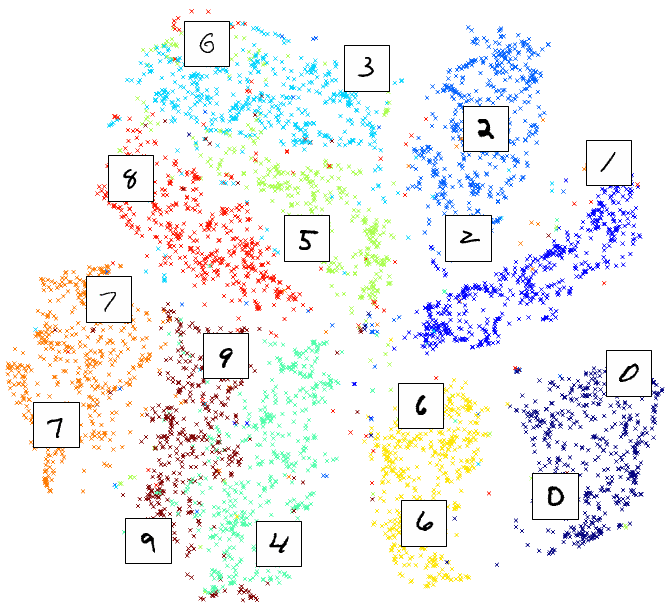
\includegraphics[scale=0.2]{tsne.png}
\caption{2D embedding of 70,000 handwritten digits (0-9) from MNIST \cite{tsne}.}
\label{tsneimg}
\end{figure}

Other methods of clustering and dimensionality reduction are also widely used for interpreting data, and although useful for gaining an intuition on relationships between features, they are not suited for explaining model behaviour as they examine only the input space itself. 

\subsection{Partial Dependence Plots}

A partial dependence plot (PDP) is a tool to demonstrate the marginal effect of one or two features on a prediction outcome. It was proposed by Friedman in 2001 to interpret and visualise the features that the proposed gradient boosting machine relied upon (though it is limited to 1 or 2 input features such that it can be displayed) \cite{pdp1}. A partial dependence function $\widehat{f_{xs}}$ can be calculated for some desired set of features S, by marginalising the model output over the set of `complement` features C (all other features):
\begin{align}
\widehat{f_{xs}}=\int \widehat{f}(x_{s}, x_{c})dP(x_{c})
\end{align}
It can be approximated with a Monte Carlo method. Friedman believed in 2001 that these might be used to help interpret ``any black box prediction method'' such as NN and SVM architectures, and that, ``[...] when there are a large number of predictor variables, it is very useful to have a measure of relevance to reduce the potentially large number of variables to be considered" \cite{pdp1}. The mentioned relevance measure was defined only in the context of the decision trees which constituted the paper's gradient boosting machine. Certainly, PDPs are suited for the low-dimensional feature spaces that were imagined in the pre-deep learning era, and are less suitable for high-dimensional input spaces such as in image classification. They are also restricted by an unrealistic assumption of independence among features.

\section{Model-Specific Methods}
Deep learning's reputation for lack of transparency has led to many attempts to explain the predictions of complex NN architectures. This section examines representative attribution methods from the backpropagation-based, gradient-based and perturbation-based approaches overviewed in Section \ref{sec:scoperesearch}, with some emphasis on those developed in the context of CNNs (i.e. image data).


\subsection{Backpropagation-Based} \label{sec:backprop}

Methods in this class try to isolate an internal model signal, such as neuron activations in a target hidden layer, and map these signals back into the input pixel space. Zeiler \& Fergus (2013) introduced the motivation for signal backpropagation as ``[...] showing what input pattern originally caused a given activation in the feature maps'' \cite{zeilerfergus2013}. 

\subsubsection{Visualising Activations - DeconvNet, Guided Backpropagation}
Visualisation of per-layer activations is one approach to explain inner model behaviour. It is different from other feature attribution approaches in that it seeks to visualise `learned features' instead of the contributions of input space features. DeconvNet and Guided Backpropagation are two popular examples of the approach and are briefly described as two forerunners of the backpropagation (and gradient) approach.

Deconvolutional networks (DeconvNet) generate backwards projections of neuron activations, by reversing individual activations during a `deconvolution' backwards-pass \cite{zeilerfergus2013}. The procedure can be summarised as passing feature map output activations as input into `deconv' layers, iteratively reversing activations and reconstructing input signals until the input pixel space is reached.

\begin{figure}[h]
\centering
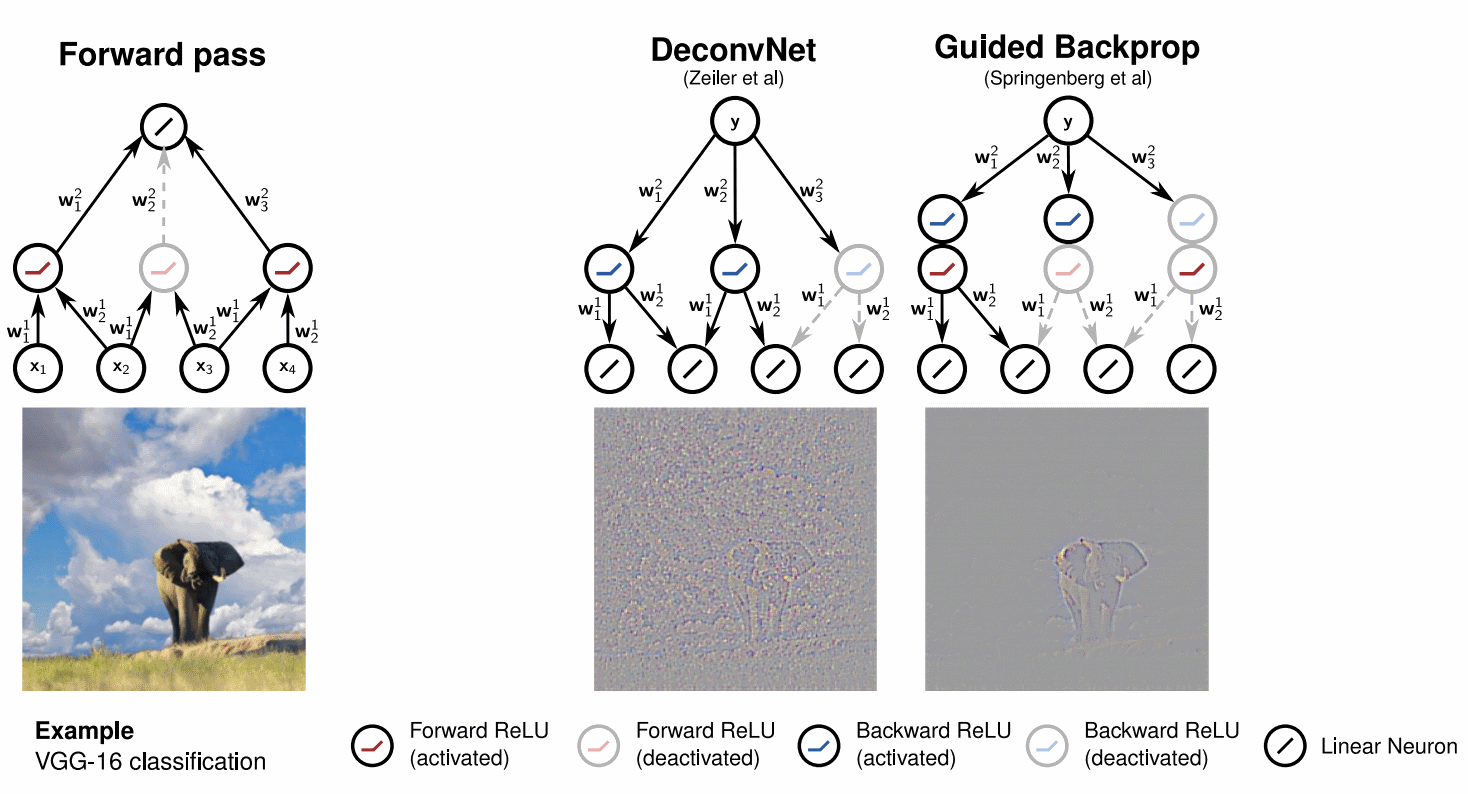
\includegraphics[scale=0.3]{deconv.png}
\caption{(Adapted from \cite{patternnet}) Illustration of DeconvNet and Guided Backprop.}
\label{deconvimg}
\end{figure}

Since it can target one layer's activation at a time, the method is useful for understanding the hierarchical learned features that CNNs generate over multiple layers. Its limitation is that during the backwards pass, it ignores any negative inputs to ReLu activations that were zero'd out in the forward pass (deactivated activations in Figure \ref{deconvimg}).

Guided Backpropagation was an enhancement by Sprigenberg et al. (2014) that added an additional signal at each step by zero'ing the importance signal if it was a negative activation in the forward pass phase \textit{or} negative in the backwards pass (the two intermediate signals in Figure \ref{deconvimg} right) \cite{springenberg}. This stopped negative gradients in lower layers from decreasing the activation of the higher layer units which were the target, and this leads to sharper explanations than those created by DeconvNet \cite{springenberg}. 

\subsubsection{DeepLIFT}

DeepLIFT (Deep Learning of Important FeaTures) \cite{deeplift} was created out of the motivation that the zero'ing of negative gradients by DeconvNet and Guided Backpropagation meant that neither are able to highlight inputs that contribute negatively to an output. In some sense they are therefore missing half the story of feature contribution. DeepLIFT's authors (Shrikumar et al. (2017)) also wanted to overcome the unaddressed saturation problem, which is that relevant neurons that contribute to a saturated output activation would not individually change the output if they were turned off (as might be tried in perturbation approaches).

DeepLIFT's innovation over previous backpropagation and gradient-based methods was to realise that where this problem existed, a single gradient value of an output with respect to an input value did not adequately or necessarily capture input contributions to an output. The authors' proposal was to find input contributions by instead calculating the absolute change in output with respect to a neuron's `reference' activation. 

\begin{figure}[h]
\centering
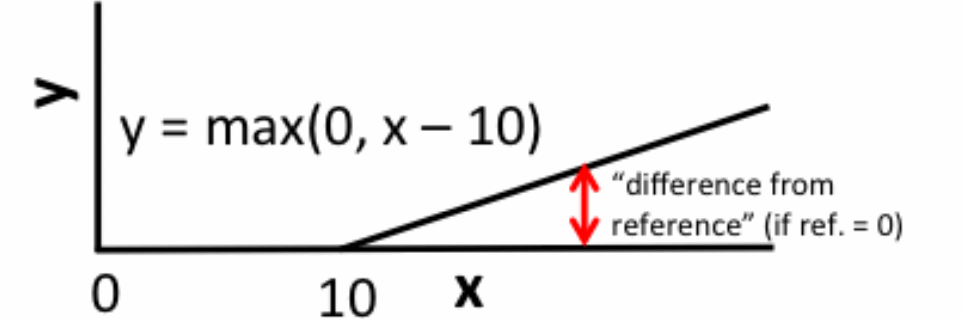
\includegraphics[scale=0.3]{deeplift.png}
\caption{(From \cite{deeplift}) Difference-from-reference attributions can avoid bias terms.}
\label{deepliftimg}
\end{figure}

Finding reference activations is an implementation difficulty. Generally, the authors propose all-zero input as a baseline (a black square for image data), and a better reference to be the average input over a background data sample \cite{deeplift}.

Like other backpropagation methods, DeepLIFT is extremely fast to calculate as it requires only a single backwards pass to propagate an importance signal back into the input space. The authors also provide different formulations for practical implementation, and a relatively high-level public implementation \cite{deepliftrepo}. The concept itself is also compatible with any NN architecture or application, unlike for example DeconvNets and Guided Backpropagation, designed for ReLu activation functions, and GradCAM (Section \textbf{X}) which was designed for CNNs.


\subsubsection{Other Backpropagation Methods}
DeepLIFT is one of several modern methods to decompose a network's prediction onto input features using activation backpropagation. For brevity its main competitors, Layerwise Relevance Propagation \cite{lrp} and DeepTaylorDecomposition \cite{taylor}, are omitted here but mentioned for the reader's reference.


\subsection{Gradient-Based} \label{sec:gradient}
These methods aim to explain a class output in terms of sensitivity in the input space by relying on a gradient function of the output\footnote{A strong overlap between gradient and backprop methods exists since gradients as derivatives are found and approximated via backprop, and the weights updated by these gradients in training/backprop are the contributions \textit{to} neuron activations.}. The goal is to find the input features that make that prediction more or less confident: for example, for an output class of `tree' they seek to answer ``what makes a tree more/less a tree?''.

\subsubsection{Saliency Maps}
An early formulation of a local explanation method was provided by Baehrens et al. (2010) for any nonlinear classification algorithm (though developed in the context of Bayesian classification) \cite{saliencyI}. The local explanation gradient vectors that this paper devised were based on class probability gradients, characterising how much a data point has to be moved for a predicted label to change.

Simonyan et al. (2014) later applied a similar idea to CNNs to create `class saliency maps' specific to a given image and class \cite{saliencyII}. 

\begin{figure}[h]
\centering
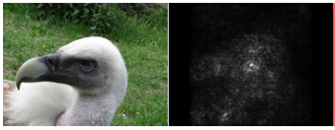
\includegraphics[scale=0.8]{saliency.png}
\caption{(From \cite{saliencyII}) Example of an image-specific class saliency map.}
\label{saliencyimg}
\end{figure}

The formulation is based on finding the derivative of an output class with respect to an input image via back-propagation. The authors also formulate a method to generate an image that maximises the output class score for a particular class, to visualise the model's `interpretation' of a class. 

%The method of computing gradients of DeconvNet-based reconstruction of the input to a hidden layer (Section 1.3.1) is equivalent to computing the gradient of visualised neuron activations with respect to that input \cite{saliencyII}.


This paper sparked great interest in CNN explanations and further interest in creating explanations from network gradients generally. Along with DeconvNet and Guided Backpropagation (developed relatively simultaneously with similar ideas) these three methods are the most historically popular and influential saliency techniques\footnote{Saliency maps are synonymous with gradient methods to the point where it is sometimes referred to as simply the `Gradients' technique, as in Adebayo et al. (2018) \cite{sanity}, who may have done so to disambiguate the technique from saliency maps generally - see Section 1.1 (``Terminology'').}. A drawback of saliency maps is that noisy images can be produced when a model does not distinguish between objects that are being predicted and nearby objects that are associated (i.e. a tree with leaves, in an image of a bird).

\subsubsection{Grad-CAM}
Class activation maps (CAMs) are another approach aimed at understanding the behaviour of CNNs introduced by Zhou et al. (2015) \cite{cam}, based on the motivation that deeper convolutional layers capture higher-level visual constructs while retaining spatial information \cite{gradcam}. While examining global average pooling (GAP) layers, a technique previously suggested for regularisation during training \cite{nin}, the authors realised a final convolutional layer's separate RGB channels (or `feature maps') could be input into a GAP layer, and then those outputs used as features in a fully-connected layer just before the final softmax layer. The class-associated weights in that fully-connected layer can be combined with the original final convolutional layer feature maps to capture deep representations as object localisations/class `activation' maps:

\begin{figure}[h]
\centering
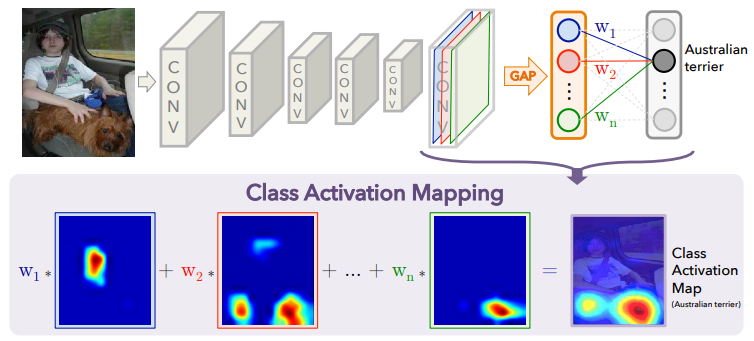
\includegraphics[scale=0.5]{cam.png}
\caption{(From \cite{cam}) Summary of the CAM formulation. RGB channels are emphasised as inputs into the weighted sum that creates a CAM.}
\label{camimg}
\end{figure}

A major limitation of the CAM approach is that it requires specific CNN architectures without previous fully-connected layers, and a GAP layer to be added before the output softmax layer to generate the deep representations it visualises. As well as this being a hurdle to adoption, the representations are highly coarse and only roughly approximate class-associated regions (a reason for their heatmap presentation).

Grad-CAM was proposed by Selvaraju et al. (2016) aimed at making CAMs applicable to a wider range of CNN models, and for visual tasks other than image classification \cite{gradcam}. It requires no alteration to model architecture. It still targets the final convolutional layer's channels, as in CAM, but uses the \textit{gradient} of an output class score with respect to these channels' output activations, to then globally-average-pool the gradients over the layer's width and height dimensions. The importance weights produced can be visualised as a localised heatmap over the input space, though the authors also combine a Guided Backpropagation output (Section \ref{sec:backprop}) with the heatmaps to generate a class-discriminative, ``high-resolution'' version called Guided Grad-CAM (Figure \ref{gradimg}).

\begin{figure}[h]
\centering
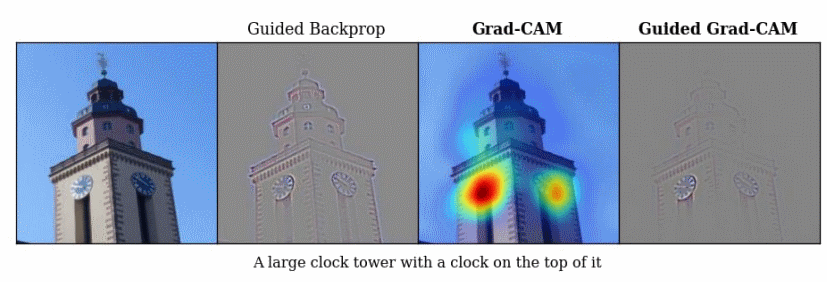
\includegraphics[scale=0.6]{gradcam_I.png}
\caption{(Adapted from \cite{gradcam}) \textit{Grad-CAM}, \textit{Guided Backprop}. and \textit{Guided Grad-CAM} on an image captioning example from the Neuraltalk2 model.}
\label{gradimg}
\end{figure}

One of Grad-CAM's strengths is that its authors prove its effectiveness for a variety of use cases. These include highlighting causes of incorrect predictions (`failure modes'), the effect of adversarial noise and causes of model confusion, and identifying training dataset bias\footnote{For example, they showed that a VGG model trained to classify nurses from doctors had learned to look at long hair to incorrectly label a female doctor a nurse, and the bias was because of gender-skewed training data.}. Its application to a variety of models by other researchers (\cite{gradcamplusplus}, \cite{xray}) is one testament to its authors' claims on cross-model applicability and explanation quality, and its popularity in the literature ($>$2000 citations). 

%gradcam efficient variation https://arxiv.org/abs/1911.11293
% gradCAM has over 2000 citations
%Occlusions for Effective Data Augmentation in Image Classification
%https://arxiv.org/abs/1910.10651
% gradCAM was also used by the introduction motivating example


\subsubsection{Other Gradient Methods}

Integrated Gradients (ref DeepLIFT) *also addresses saturation

SmoothGrad



%Understanding Deep Networks via Extremal Perturbations and Smooth Masks
%https://arxiv.org/abs/1910.08485

%Interpretable Explanations of Black Boxes by Meaningful Perturbation
%http://openaccess.thecvf.com/content_ICCV_2017/papers/Fong_Interpretable_Explanations_of_ICCV_2017_paper.pdf


%<put figure in comparing gradient and backprop ones i.e. deep %explainer or patternattribution>

\subsection{Perturbation-Based}

occlusion and ablation

occlusion mask, zeiler and fergus


\subsection{Other NN Techniques}

Some model-specific methods which do not attribute the contribution of features, or project internal model signals onto the input space, may also be of interest to the reader. These include Net2CV, mentioned in Section 1.X .

\section{Model-Agnostic Methods}


"While we have made a case for model agnosticism, this
approach is not without its challenges. For example,
getting a global understanding of the model may be hard
if the model is very complex, due to the trade-off between
flexibility and interpretability. To make matters worse, local
explanations may be inconsistent with one another, since a
flexible model may use a certain feature in different ways
depending on the other features. In Ribeiro et al. (2016)
we explained text models by selecting a small number
of representative and non-redundant individual prediction
explanations obtained via submodular optimization, similar
in spirit to showing prototypes (Kim et al., 2014). However,
it is unclear on how to extend this approach to domains such
as images or tabular data, where the data itself is not sparse.
In some domains, exact explanations may be required (e.g.
for legal or ethical reasons), and using a black-box may
be unacceptable (or even illegal). Interpretable models
may also be more desirable when interpretability is much
more important than accuracy, or when interpretable models
trained on a small number of carefully engineered features
are as accurate as black-box models."  Model-Agnostic Interpretability of Machine Learning



\subsection{Perturbation-Based}
Both gradient and backpropagation-based methods operate under the assumption that propagating an output signal, back through a classifier model, is a means to explain how a relevant signal was originally encoded in an input \cite{patternnet}. An alternative approach is to treat the model as more of a black box, by perturbing the input space (such as occluding important parts) to study the effect on the output. Changes in output would reveal that occluded parts of the input are important in a prediction. 

"The problem of attribution is concerned with identifying the parts of an input that are responsible for a model's output. An important family of attribution methods is based on measuring the effect of perturbations applied to the input"




\subsection{Surrogate Models}
some overlap with perturbation-based methods for how they are trained

%https://christophm.github.io/interpretable-ml-book/lime.html


variants of lime include KL-lime

\section{Evaluation Metrics}

\subsection{What makes a visual explanation a quality one?}
% gradcam paper "What makes a good visual explanation?"


%https://arxiv.org/abs/1907.09701
%https://distill.pub/2020/attribution-baselines/

%https://arxiv.org/pdf/1711.00867.pdf

%sanity checks for saliency maps
%https://arxiv.org/pdf/1810.03292.pdf

%unreliability of saliency methods
%https://arxiv.org/pdf/1711.00867.pdf

%https://medium.com/swlh/breaking-down-the-black-box-39403b0f64a3

%IOU: Network Dissection: Quantifying Interpretability
%https://arxiv.org/abs/1704.05796

%\cite{saliencyII}
%Section 3.2 Weakly Supervised Object Localisation
%weakly supervised object localisation from Saliency Maps
%used a segmentation algorithm and entered their saliency
% map into ILSVRC-2013 localisation challenge

%http://cnnlocalization.csail.mit.edu/Zhou_Learning_Deep_Features_CVPR_2016_paper.pdf
% CAM authors also test CAMs on object localisation without bounding box annotation %"Weakly-supervised object localization"

\section{Existing Explanation Frameworks}


%TreeExplainer repo??


%Skater - a unified framework for model-agnostic interpretation --> global and local
%DeepExplainer

%TorchRay https://github.com/facebookresearch/TorchRay

\section{Existing Evaluation Studies}

Comparisons

% https://openreview.net/forum?id=Sy21R9JAW
% pytorch
% deepexplainer


\end{document}
